% ============================================================================
%  fastpiclef --- readable technical report (docs/report/main.tex)
%
%  Build:   latexmk -pdf main.tex        (pdflatex, TikZ)
%  Status:  first draft (2026-10-13).  Numbers marked [pending: ...] are
%           intentionally unfilled until the final measurement pass on a quiet
%           machine; everything else is dataset-backed (see Appendix B).
% ============================================================================
\documentclass[11pt,a4paper]{article}

\usepackage[a4paper,margin=2.5cm]{geometry}
\usepackage[utf8]{inputenc}
\usepackage[T1]{fontenc}
\usepackage{lmodern}
\usepackage{amsmath,amssymb}
\usepackage{graphicx}
\usepackage{array}
\usepackage{url}
\usepackage{booktabs}
\usepackage{microtype}
\usepackage{xcolor}
\usepackage{tikz}
\usetikzlibrary{arrows.meta}
\usepackage[colorlinks=true,linkcolor=blue!50!black,citecolor=blue!50!black,
            urlcolor=blue!50!black]{hyperref}
% \usepackage{natbib}

\newcommand{\pending}[1]{\textcolor{red}{[pending: #1]}}
\setlength{\emergencystretch}{1.5em}
\DeclareUrlCommand\code{\urlstyle{tt}}
\newcommand{\Fresnel}{F}
\newcommand{\ii}{\mathrm{i}}
\newcommand{\dd}{\mathrm{d}}
\newcommand{\R}{\mathbb{R}}
\newcommand{\C}{\mathbb{C}}
\newcommand{\ie}{i.e.}
\newcommand{\eg}{e.g.}

\graphicspath{{../../comparison/results/}{figures/}}

\title{\bfseries Fast Picard--Lefschetz evaluation of the lensing Fresnel
integral\\[2mm]
\large The \texttt{fastpiclef} solver: methods, validation, and performance}
\author{Paul\\[1mm]
\small with development sessions (\texttt{opencode})}
\date{Draft --- \today}

\begin{document}
\maketitle

\begin{abstract}
\noindent
Wave-optics gravitational lensing replaces the geometric-optics sum over
images by a two-dimensional Fresnel integral,
$\Fresnel(\omega,\boldsymbol{\beta}) \propto \int_{\R^2}
e^{\ii\omega\varphi(x;\boldsymbol{\beta})}\dd^2x$, whose direct evaluation is
numerically hostile: the integrand oscillates on the Fresnel scale
$1/\sqrt{\omega}$, the integral converges only conditionally at infinity, and
point-mass lenses add logarithmic branch points that real-space quadratures
cannot cross.  This report describes \texttt{fastpiclef}, a Rust core with a
Python interface that evaluates this integral \emph{exactly} (to machine
precision, with a validated error budget) by deforming the contour into the
complex plane along Picard--Lefschetz steepest-descent directions, organised
as a real core anchored at every branch-point pinch plus $\pi/4$-rotated
Gaussian-decay tails, applied recursively in the two integration variables.
We describe the model class (point masses, external convergence and shear,
and circular lens profiles), the solver family (the exact 2D ``rotated
contour'' engine, a 1D thimble solver, an axisymmetric referee, a
Nakamura--Deguchi closed form, batched sweeps/maps/grids, and a high-$\omega$
geometric-plus-correction hybrid), the validation methodology (external
referees, independent contour families, bitwise baselines --- self-agreement
is explicitly not accepted as truth), and the measured performance against
the reference codes \texttt{plind}, \texttt{P-LPI}, and FIONA.  The solver
reaches $10^{-15}$-class accuracy against independent closed forms across
$\omega \in [0.3, 1000]$ for point-mass fields, is exact also on saddle-type
macro images where real-box methods fail by $29$--$49\%$, and amortises
source grids and frequency sweeps through shared-contour batching and
deterministic parallelism.
\end{abstract}

\tableofcontents

% ============================================================================
\section{Introduction}
\label{sec:intro}

\subsection{Wave-optics gravitational lensing}
\label{sec:physics}

When the wavelength of radiation passing a gravitational lens is not
negligible compared with the geometric lensing scales, the geometric-optics
description (images, magnifications, caustics) is replaced by diffraction:
the observed amplification is a coherent sum over all paths, \ie{} a Fresnel
integral over the lens plane.  Writing $x$ for the (two-dimensional) image
position, $\boldsymbol\beta$ for the source position, and
\begin{equation}
  \varphi(x;\boldsymbol\beta)
  \;=\; \tfrac12\,|x-\boldsymbol\beta|^2 \;-\; \psi(x)
  \label{eq:fermat}
\end{equation}
for the Fermat potential of the lens $\psi$ (lengths in units of a reference
Einstein radius), the amplification factor in the standard normalisation is
\begin{equation}
  \Fresnel(\omega,\boldsymbol\beta)
  \;=\; \frac{\omega}{2\pi\ii}\int_{\R^2}
  e^{\ii\,\omega\,\varphi(x;\boldsymbol\beta)}\,\dd^2 x,
  \label{eq:fresnel}
\end{equation}
so that free space ($\psi \equiv 0$) gives $\Fresnel = 1$ and the observed
flux magnification is $|\Fresnel|^2$ \cite{DeguchiWatson1986,Nakamura1998,TakahashiNakamura2003}.
The dimensionless frequency is
\begin{equation}
  \omega \;=\; \frac{8\pi G M_{Lz} f}{c^3}
  \;\approx\; 1.2379\times 10^{-4}\;
  \frac{M_{Lz}}{M_\odot}\,\frac{f}{\mathrm{Hz}},
  \label{eq:omega}
\end{equation}
with $M_{Lz}$ the lens mass inside the line of sight and $f$ the wave
frequency.  The science regimes of interest span a wide range:

\begin{center}
\small
\begin{tabular}{@{}>{\raggedright\arraybackslash}p{6.2cm}lll@{}}
\toprule
setting & $M_{Lz}$ & $f$ & $\omega$ \\
\midrule
ground interferometers (LVK/ET/CE) $\times$ stellar lenses
  & $0.1$--$100\,M_\odot$ & $10$--$1000$\,Hz & $10^{-4}$--$12$\\
LISA $\times$ haloes and subhaloes
  & $10^{3}$--$10^{9}\,M_\odot$ & $10^{-4}$--$0.1$\,Hz & $10^{-5}$--$10^{4}$\\
\bottomrule
\end{tabular}
\end{center}

In the geometric limit $\omega\to\infty$, Eq.~\eqref{eq:fresnel} reduces to
the familiar sum over the stationary points $x_i$ of $\varphi$,
\begin{equation}
  \Fresnel_{\rm geo}(\omega)
  \;=\; \sum_i |\mu_i|^{1/2}\,
  e^{\ii\left(\omega\,\varphi(x_i) - \pi n_i\right)},
  \qquad n_i \in \{0,\tfrac12,1\},
  \label{eq:geo}
\end{equation}
where $\mu_i = 1/\det \partial^2\varphi(x_i)$ is the (signed) magnification
and $n_i$ is the Morse index of the image ($0$ minimum, $\tfrac12$ saddle,
$1$ maximum).  Wave optics matters precisely where this replacement is
invalid: near caustics, where images coalesce, and at the moderate
frequencies (1) of stellar-mass lenses seen by ground-based detectors.

\subsection{What this code computes}
\label{sec:what}

\texttt{fastpiclef} evaluates Eq.~\eqref{eq:fresnel} \emph{without any
asymptotic approximation} for the model class of Sec.~\ref{sec:model} ---
point masses, an external convergence $\kappa$ and shear
$(\gamma_1,\gamma_2)$, and circular lens profiles --- returning a complex
value and a conservative error estimate for every call.  The validated range
for point-mass fields is $\omega \in [0.3, 1000]$ over the source plane up
to the far tails of the field; harder quantities (saddle-type macro images,
many-component fields, high $\omega$) have dedicated paths described in
Sec.~\ref{sec:engines}.  The Python surface is a thin layer over the Rust
core:
\begin{quote}\ttfamily
import fastpiclef as fpl\\
lf = fpl.LensField([fpl.PointComp(0.3, 0.0, 1.0)], beta=(0.1, 0.0), kappa=0.2)\\
r\ \ =\ lf.solve(omega=10.0)\ \ \# exact RC path by default\\
r.amplification,\ r.error\ \ \# complex value, conservative error
\end{quote}
Batched evaluation (\texttt{sweep}, \texttt{map}, \texttt{grid}) shares one
contour across a family of frequencies or source positions; geometric optics,
image finding, and a high-$\omega$ asymptotic branch are exposed on the same
objects.

\subsection{Strategy in one paragraph}
\label{sec:strategy}

The core idea is a \emph{Cauchy deformation}: because the integrand of
Eq.~\eqref{eq:fresnel} is analytic in $x$ (except at the lens's branch
points), the domain of integration may be moved into the complex plane,
where the oscillatory factor $e^{\ii\omega\varphi}$ becomes a product of a
Gaussian decay and a bounded phase.  The practical contour we use ---
described in Sec.~\ref{sec:method} and illustrated in
Fig.~\ref{fig:contour} --- is a \emph{real core} in each integration
variable, anchored at every branch-point pinch so that no panel spans a
singularity, plus two $\pi/4$-rotated tails on which the Gaussian factor
$e^{-\omega|\lambda|s^2/2}$ decays.  This is a Picard--Lefschetz
steepest-descent construction in the sense of the standard literature
\cite{Feldbrugge2019,Jow2021,Shi2024}, organised for exactness and
robustness rather than for thimble bookkeeping: no cancellation is left in
the integrand, no homology tracking is needed, and the result is exact by
Cauchy, with an error budget assembled from panel differences, propagated
inner integrals, and tail truncation.

\subsection{Scope of this report}
\label{sec:scope}

This report is the readable companion to the code base.  It is written for a
reader with a lensing background but no familiarity with complex
steepest-descent quadrature, and it aims to be honest about costs and
limits: every quantitative claim below names the dataset that supports it
(Appendix~\ref{app:map}), and measurements are quoted with the machine load
when wall-clock times are involved.  Derivation-level details live in the
code's module documentation and tests, and the complete catalogue of error
sources and their budgets is the companion document
\code{docs/error_budget.md}.

% ============================================================================
\section{Why the direct integral is hard}
\label{sec:hard}

\subsection{Oscillation and conditional convergence}

For large $\omega$ the integrand of Eq.~\eqref{eq:fresnel} oscillates on the
Fresnel scale $\sim 1/\sqrt{\omega}$ while the integrand itself decays only
because of the quadratic term.  Two numerical facts rule out naive
quadrature:

\begin{enumerate}
\item \emph{Cancellation.}  The integral is a sum of terms of size $\sim
  \omega^{-1}$ whose result can be much smaller; resolving it to a relative
  accuracy of $\epsilon$ requires the phase to be tracked far below
  $\epsilon$ in absolute terms.  The integrand also never dies: along the
  real axes its modulus is non-decaying, so contribution- and
  error-estimates cannot be based on decay.
\item \emph{Conditional convergence.}  Cutting the plane at radius $R$
  leaves a boundary term of relative size
  $\sim 1/(\omega R^2)$ with a wildly oscillating phase
  ($e^{\ii\omega R^2/2}$): reaching$10^{-15}$ accuracy by truncation would
  need $\omega R^2 \gtrsim 10^{15}$.  Real-space windows \emph{can be} made
  to work at fixed accuracy by design (that is what FFT-based codes do), but
  the truncation is a systematic error that cannot be inferred from the
  inside, and it fails outright in the saddle-image geometry of
  Sec.~\ref{sec:saddle}.
\end{enumerate}

\subsection{Caustics}
\label{sec:caustics}

The physically interesting regime is near caustics, where two or more
stationary points of $\varphi$ coalesce.  There the second-derivative
(Hessian) description breaks down, $(2\pi/\omega)^{1/2}$-type asymptotics
fail, and the Fresnel integral smoothly interpolates between the
geometric-optics branches --- the classic Airy-interference regime.  A
production solver must handle image pairs that are closer than the Fresnel
scale, {\it without} the quadrature silently losing them: the management of
near-degenerate stationary points is a structural requirement, not a corner
case.

\subsection{Saddle images: conditionally convergent directions}
\label{sec:saddle}

A macro image where the Fermat potential has eigenvalues of \emph{opposite}
sign (a saddle point; $n = \tfrac12$ in Eq.~\eqref{eq:geo}) is the hardest
geometry for real-space methods: along one real direction the phase is
locally a maximum, so the integrand grows for a while before the global
quadratic term dominates; the integral converges only conditionally and the
convergence is not uniform in the saddle location.  This is not a technical
curiosity: for the saddle-type macro image case the FFT-based reference code
FIONA errs by $29$--$49\%$ even for the trivial lens-free check where the
answer is $|\Fresnel| = 1/\sqrt{|\lambda_0\lambda_2|}$ exactly (dataset:
\code{comparison/results/fiona_grid.csv}, and the saddle macro-image
tests).  Our solver is exact there ($\lesssim 6\times10^{-15}$ on the same
cases) because the Cauchy-deformed contour decays \emph{in all directions by
construction}.

\subsection{Logarithmic branch points of point-mass lenses}
\label{sec:branches}

Point-mass lenses have $\psi(x) = \sum_j m_j \ln|x-a_j|$, whose logarithm
becomes a branch point in the complexified coordinates.  In the
slice-by-slice organisation of Sec.~\ref{sec:method} each mass contributes a
\emph{pinch}: a height $x_2 = b_j$ at which the two branch points of that
component meet on the integration contour.  A usable deformation must
therefore (i) anchor its quadrature panels exactly at the pinches, (ii) keep
every integration path clear of the branch cuts, and (iii) leave the result
independent of the deformation parameters --- which the code verifies
explicitly by running an independent contour family (Sec.~\ref{sec:val}).

\subsection{And it has to be fast}

A single value is rarely the deliverable: applications need
\texttt{map}s over the source plane, \texttt{sweep}s over frequency, and
grids over both, for fields with up to many dozens of point masses.  The
design therefore separates \emph{exactness machinery} (contour construction,
anchoring, budgets) from \emph{amortisation} (shared contours, batched
twiddles, deterministic parallelism) --- these are the subjects of
Secs.~\ref{sec:method} and \ref{sec:engines}, with performance in
Sec.~\ref{sec:perf}.

% ============================================================================
\section{The method: Cauchy deformation and the RC construction}
\label{sec:method}

\subsection{Picard--Lefschetz in one picture}

For an integral $\int_{\R^d} e^{\ii\omega\varphi(x)}\dd^dx$ with $\omega$
large, consider the complexification of $\varphi$.  Its stationary points
(images) are saddle points of $\Re(\ii\varphi)$; through each passes a
steepest-descent manifold (a Lefschetz thimble) along which
$\Re(\ii\varphi)$ decreases monotonically, so the integrand decays
exponentially away from the stationary point.  The integral over the real
domain can be deformed (by Cauchy's theorem) onto the union of thimbles,
each weighted by an integer intersection number; along the way, oscillations
are traded for exponential decay and the quadrature becomes tame.  This is
the classical Picard--Lefschetz route to diffraction integrals
\cite{Feldbrugge2019,Jow2021,Shi2024}, and it has to be executed carefully:
the deformation is only as good as the bookkeeping of which thimbles are
picked up, and near branch points the ``thimbles'' change topology.

Our construction takes the same physical idea --- oscillate $\to$ decay ---
but arranges the contour so that no bookkeeping is required at all.  The
integrand is analytic in each variable separately in a large region whose
boundary (for point masses) consists of the branch cuts of the logarithms.
Inside that region we choose one fixed, explicitly parametrised contour
family and use Cauchy's theorem to assert that its value equals the real
integral's.  Contour independence is then verified empirically by varying
the family (the ``$\alpha$-family'', below), which is cheap and decisive.

\begin{figure}[t]
\centering
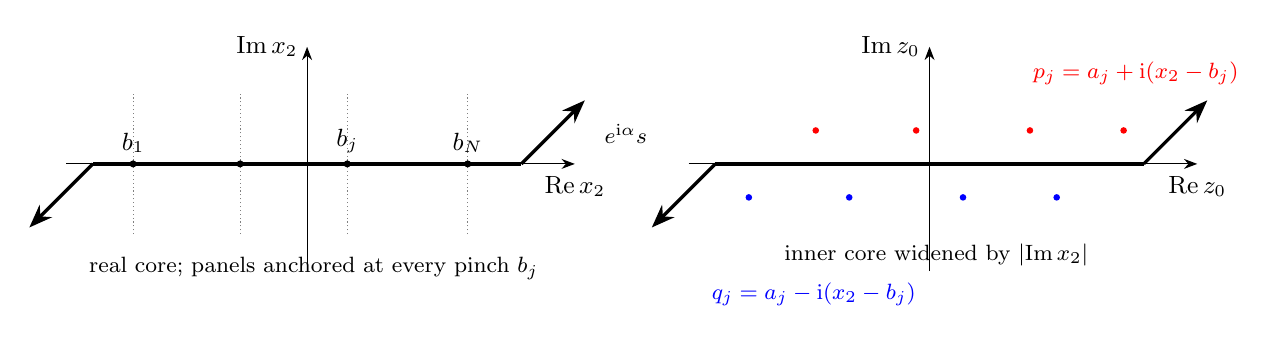
\begin{tikzpicture}[scale=0.85,font=\small,>=Stealth]
% ---------------- outer variable ------------------------------------------
\begin{scope}
  \draw[->] (-3.6,0) -- (4.0,0) node[below,yshift=-1pt] {$\mathrm{Re}\,x_2$};
  \draw[->] (0,-1.6) -- (0,1.75) node[left] {$\mathrm{Im}\,x_2$};
  % branch cuts (schematic)
  \foreach \x in {-2.6,-1.0,0.6,2.4}{
    \draw[densely dotted,gray] (\x,-1.05) -- (\x,1.05);
    \fill (\x,0) circle (1.5pt);
  }
  % core
  \draw[very thick] (-3.2,0) -- (3.2,0);
  % tails
  \draw[very thick,->] (3.2,0) -- (4.15,0.95);
  \draw[very thick,->] (-3.2,0) -- (-4.15,-0.95);
  \node[above] at (-2.6,0.02) {$b_1$};
  \node[above] at (0.6,0.02) {$b_j$};
  \node[above] at (2.4,0.02) {$b_N$};
  \node[anchor=north,align=center,font=\footnotesize] at (0.1,-1.25)
      {real core; panels anchored at every pinch $b_j$};
  \node[anchor=west,align=left,font=\footnotesize] at (4.3,0.45)
      {$e^{\ii\alpha}s$};
\end{scope}
% ---------------- inner variable ------------------------------------------
\begin{scope}[xshift=9.3cm]
  \draw[->] (-3.6,0) -- (4.0,0) node[below,yshift=-1pt] {$\mathrm{Re}\,z_0$};
  \draw[->] (0,-1.6) -- (0,1.75) node[left] {$\mathrm{Im}\,z_0$};
  \draw[very thick] (-3.2,0) -- (3.2,0);
  \draw[very thick,->] (3.2,0) -- (4.15,0.95);
  \draw[very thick,->] (-3.2,0) -- (-4.15,-0.95);
  % branch points for a complex x2: two families, one per sign
  \foreach \x in {-2.2,-0.7,1.0,2.4}{
    \fill[red] (\x+0.5,0.5) circle (1.4pt);
    \fill[blue] (\x-0.5,-0.5) circle (1.4pt);
  }
  \node[red,anchor=west,font=\footnotesize] at (1.4,1.35)
      {$p_j = a_j + \ii(x_2-b_j)$};
  \node[blue,anchor=west,font=\footnotesize] at (-3.4,-1.95)
      {$q_j = a_j - \ii(x_2-b_j)$};
  \node[anchor=north,align=center,font=\footnotesize] at (0.1,-1.05)
      {inner core widened by $|\mathrm{Im}\,x_2|$};
\end{scope}
\end{tikzpicture}
\caption{Schematic of the rotated-contour (RC) construction, drawn in the
outer variable $x_2$ (left) and the inner variable $z_0$ (right) of the
two-variable integral.  In each variable the contour is a real core --- with
quadrature panels anchored at every pinch so no panel spans a singularity
--- plus two tails rotated by $\pm\pi/4$ (sign chosen per macro eigenvalue),
on which the Gaussian factor decays like $e^{-\omega|\lambda|s^2/2}$.
Dotted vertical lines sketch the branch cuts of the point-mass logarithms;
after rotation the cuts are never crossed.  The same construction applies one
level down: for a complex outer node $x_2$, the inner integrand has two
branch-point families $p_j, q_j$ that follow $x_2$ rigidly, and the inner
core widens by $|\mathrm{Im}\,x_2|$ so that both families stay inside it.
The result is exact by Cauchy; $\alpha\in(0,\pi/4]$ (the tail angle) is a
free parameter whose variation is used as an independent check.}
\label{fig:contour}
\end{figure}

\subsection{The RC construction, precisely}

In the ``diagonal shear'' coordinates of Sec.~\ref{sec:model} the phase
splits as
\begin{equation}
\varphi(x_0,x_2) = \tfrac12\lambda_0 x_0^2 - \beta_0 x_0
  + \tfrac12\lambda_2 x_2^2 - \beta_1 x_2
  + \tfrac12|\boldsymbol\beta|^2
  - \sum_j \psi_j\!\left(w_j\right),
\qquad
w_j = (x_0-a_j)^2 + (x_2-b_j)^2 ,
\label{eq:split}
\end{equation}
with $\lambda_0 = 1-\kappa-\gamma$, $\lambda_2 = 1-\kappa+\gamma$ and the
(for our model class) analytic profile functions $\psi_j$ of the complex
quadratic form $w_j$.  The two-variable integral is organised as an outer
integral in $x_2$ whose integrand is, for each $x_2$, a complete inner
integral in $x_0$:
\begin{equation}
\Fresnel = \frac{\omega}{2\pi\ii}\int_{\text{outer}}
e^{\ii\omega\left(\frac12\lambda_2 x_2^2-\beta_1x_2\right)}
\left[\int_{\text{inner}(x_2)}
e^{\ii\omega\left(\frac12\lambda_0 x_0^2-\beta_0 x_0
  -\sum_j\psi_j(w_j)\right)}\dd x_0\right]\dd x_2 .
\label{eq:nested}
\end{equation}
Each of the two integrals gets the same treatment:

\begin{itemize}
\item \textbf{Real core, anchored.}  The core of the outer variable runs
  along the real axis covering every pinch height $b_j$ (each mass
  contributes one) and every Gaussian centre $\beta_1/\lambda_2$;
  \emph{panels are anchored at the pinches}, and the two half-intervals
  around a pinch are parametrised as $x_2 = b_j \pm \rho^2$, which makes the
  mildly cuspy integrand quadrature-smooth.  The inner core runs along the
  real $z_0$ axis covering every branch-point abscissa --- which for a
  complex outer node $x_2$ includes the widened positions
  $a_j \mp \mathrm{Im}(x_2-b_j)$ --- and the Gaussian centre
  $\beta_0/\lambda_0$.  The inner core consequently widens linearly with
  $|\mathrm{Im}\,x_2|$.
\item \textbf{Rotated tails.}  From the ends of each core, the contour
  continues along $x = \text{end} + \sigma\, e^{\ii\theta} s$, with
  $\theta = \mathrm{sgn}(\lambda)\,\alpha$, $\alpha \in (0,\pi/4]$
  (default $\alpha = \pi/4$), $\sigma = \pm1$.  Because the quadratic term
  along these rays has $\Re(\ii\lambda x^2/2) \to -\infty$, the integrand
  decays like $e^{-\omega|\lambda| s^2/2}$; the tail length uses the largest
  Gaussian that still resolves the $\omega_{\min}$ of the batch, plus a
  decay probe with a truncation budget.
\item \textbf{Cuts are respected.}  Along the whole contour each $w_j$
  stays in a closed quadrant that excludes the negative real axis (where
  the profile functions are cut), so the profile functions are evaluated on
  their principal branches without crossing cuts; the author's pen-and-paper
  argument is reproduced in the code's module documentation and confirmed
  numerically by the $w$-quadrant checks.  Mixed-sign macro cases (saddle
  images) keep $\Re w_j > 0$ strictly.  \emph{Not} allowed: $\alpha > \pi/4$,
  which can cross a cut in the mixed-sign case.
\item \textbf{Exactness.}  With the cuts avoided, Cauchy's theorem makes the
  value independent of the (positive) core extents, the tail angle, and the
  tail length.  Nothing in the construction is asymptotic: the quadrature
  simply integrates the (now non-oscillatory, exponentially decaying)
  integrand.
\end{itemize}

The free parameters turn into the solver's own quality control: the
\emph{$\alpha$-family} ($\pi/4$ vs $\pi/8$) and independent \emph{margins}
$B$ are run in tests and in the reference layer as independent contour
families; their agreement (typically $10^{-15}$--$10^{-14}$) is the
strongest routine evidence that no cut was crossed and no contribution was
lost.

\subsection{Budgets}
\label{sec:budgets}

Every returned value carries a conservative error estimate assembled from:
per-panel embedded-quadrature differences (Gauss--Legendre with a
20-node panel and its two 10-node halves), propagation of the inner
integral's own budget through the outer Jacobian at every outer node, tail
truncation (probed decay, budgeted by the last integrand value times the
remaining length), roundoff floors set at the ulp level of the phase
$\omega\varphi$, and panel caps with an explicit ``capped'' flag.  The
1D kernels add a homology-completeness indicator (a branch point swept
between adjacent slices) with a $100\times$ safety factor, itself validated
against measured errors.  The full catalogue, term by term, is
\code{docs/error_budget.md}; Sec.~\ref{sec:val} describes how the budgets
are validated rather than trusted.

% ============================================================================
\section{The solver family}
\label{sec:engines}

The repository ships several engines that share the conventions above and
cross-validate each other.  Table~\ref{tab:engines} summarises the roles;
the paragraphs below give the when-and-why.

\begin{table}[t]
\centering
\footnotesize
\setlength{\tabcolsep}{4pt}
\begin{tabular}{@{}p{2.35cm}p{2.15cm}p{3.25cm}p{3.35cm}p{3.0cm}@{}}
\toprule
engine & problem & model & character & role\\
\midrule
\texttt{slice\_field} (RC, 2D) & Eq.~\eqref{eq:fresnel} & point masses $+$
  macro $+$ circular profiles & exact, budgeted & production\\
\texttt{ThimbleSolver} (1D) & 1D Fresnel & rational phases & exact
  (complete saddle source) & 1D lenses; cross-checks\\
\texttt{Solver<D>} (mesh flow) & any $d$ & generic phases & iterative,
  oracle-grade & fallback; validation oracle\\
polar path & axisymmetric & point mass, SIS/CIS/NFW & exact (1D reduction)
  & referee; fast high-$\omega$ path\\
\texttt{point\_mass\_nd} & isolated point mass & closed form & exact to
  $|z|\lesssim10$ & $\mu$s-class fast path\\
batched paths & grids/sweeps & as above & shared contours,
  bitwise-parallel & maps, sweeps, parameter grids\\
geometric $+$ correction & $\omega\to\infty$ & any images & asymptotic with
  budget & high-$\omega$ hybrid\\
geometric (images) & any & point-mass fields & $O(\#\text{images})$,
  exact-step finder & macro model; fallback\\
\bottomrule
\end{tabular}
\caption{The solver family.  The production exact path is the 2D RC engine;
everything else either feeds it (image finding, fast paths) or checks it
(referees, oracles).}
\label{tab:engines}
\end{table}

\subsection{The exact 2D RC engine (production path)}
The engine of Sec.~\ref{sec:method} is the default for
\texttt{PointMassField} and \texttt{LensField}: any number of point masses,
a macro convergence/shear, and circular profiles, at any source position
(including the caustic-adjacent and saddle-image geometries), for
$\omega \in [0.3, 1000]$ in the validated range.  Its cost is dominated by
the number of quadrature panels, which grows with the number of pinches
($\propto N$ for $N$ masses) and with $\omega$ like a power law
(Sec.~\ref{sec:perf}).

\subsection{Thimbles in one dimension}
The 1D solver deforms onto thimbles attached to saddles of a rational
phase, where the complete saddle set is known analytically
(\texttt{RationalPhase}), giving machine-precision values for the
one-dimensional lens models used as test problems; a hybrid path falls back
to the general mesh-flow solver when a trace stalls.  This engine is also
the reference for the 2D code on sliced problems (e.g.\ the rational-lens
$\kappa=-2$ benchmarks of Sec.~\ref{sec:head2head}).

\subsection{The mesh-flow solver}
The original \texttt{Solver<D>} follows a Picard--Lefschetz flow on a mesh
and integrates where the flow settles; it works for generic phases and
arbitrary dimension but is slow, has no machine-precision guarantee, and
diverges for log potentials (exactly our point masses).  It survives as an
\emph{oracle} for cross-checks and as a fallback inside hybrid paths ---
never as the production path.

\subsection{Axisymmetric referee and closed form}
For a single point mass (or a circular profile) the problem is
axisymmetric, and a high-precision polar reduction provides an independent
referee at dozens of digits, used throughout the test suite.  For the
isolated point-mass lens there is also the Nakamura--Deguchi closed form
\cite{Nakamura1998,TakahashiNakamura2003} evaluated in log space
(\texttt{point\_mass\_nd}): $\mu$s-class at $10^{-15}$--$10^{-13}$ while
$|z| = \omega y^2/2 \lesssim 6$ and degrading like $\varepsilon e^{|z|}$
beyond, with the honest band $|z| \lesssim 10$ and a conservative returned
estimate.  Fast-path guidance: low $\omega$ $\to$ ND, else the exact RC;
high $\omega$ $\to$ the polar path ($\sim$30\,ms at $\omega=10$,
$\sim$300\,ms at $\omega=100$), then ND.

\subsection{Batched evaluation}
Sources grids, frequency sweeps and parameter grids are the actual
deliverables of a survey, and they share almost all of the work: the source
dependence factors out of the expensive pseudo-differential part of the
integrand (a twiddle per node), and frequency families can share one contour
sized for their hardest member (bands with $\omega_{\max}/\omega_{\min}
\le 10$).  The result is one contour construction amortised over many right-
hand sides --- measured $13\times$ at $N=100$ masses on a $4\times4$ source
grid (Sec.~\ref{sec:perf}).  Batched evaluation is \emph{bitwise identical}
to per-point evaluation (fixed node and reduction order, pinned by
bitwise-baseline tests), and parallelism is deterministic: threads are used
at the level of independent contour tasks, not inside reductions.

\subsection{High-\texorpdfstring{$\omega$}{omega} hybrid}
For very high $\omega$ (halo lenses at LISA: $\omega \lesssim 10^4$), even
the deformed contour becomes expensive (cost $\sim\omega^{1.45}$,
Sec.~\ref{sec:perf}), while geometric optics plus a first correction is
excellent: the solver can return
\begin{equation}
  \Fresnel = \sum_j G_{0,j}\left(1 + \frac{C_j}{\ii\omega}\right),
  \qquad
  G_{0,j} = |\mu_j|^{1/2} e^{\ii(\omega\varphi_j-\pi n_j)},
  \label{eq:hybrid}
\end{equation}
the next-order stationary-phase correction $C_j$ being expressible from the
Fresnel-region expansion of the phase around each image.  The branch is
selected only when the reported budget
$3\sum_j |G_{0,j}||C_j|/\omega$ fits the caller's tolerance (default
\texttt{tol} keeps the exact engine on the $10^{-9}$ path); the raw estimate
covered the corrected residual by $\ge 3.5\times$ in every measured family,
so the budget keeps a $\ge 10\times$ margin on the measured minimum
(dataset: \code{comparison/results/hybrid_check.csv}).  At a caustic
($|\det\partial^2\varphi| < 10^{-12}$) the branch refuses and the exact
engine takes over.  One caveat is structural: the budget bounds the
\emph{asymptotic} error at the images it found, not the existence of a
missing image; the Newton image finder is therefore dense ($24\times24$,
golden-ratio jittered) and residual-verified --- installed after a silent
miss was found (the faint image of the unit point mass at $y=1$: a $9.6\%$
error inside a $1.5\times10^{-3}$ budget with an aligned $8\times8$ start
grid).  Point-mass-only entry points use the polynomial-complete
Witt--Mao finder instead.

\subsection{Geometric optics and image finding}
The geometric sum of Eq.~\eqref{eq:geo} and the images themselves are
exposed for macro modelling and as a fallback at high $\omega$, with an
honest zero error by definition (it is an asymptote, not a quadrature).  A
tempting completeness certificate --- the signed-magnification sum rule ---
was tested and \emph{rejected}: it fails for multi-point-mass fields
($0.877$ for a three-mass case) and for cuspy or infinite-mass profiles
(SIS: $2.000$; NFW: $2.01$).

% ============================================================================
\section{The model class}
\label{sec:model}

After rotating coordinates so that the external shear is diagonal
($\gamma = \sqrt{\gamma_1^2+\gamma_2^2} = \mathrm{sgn}(\gamma_1)\gamma_1$,
$\theta_\gamma = \tfrac12\operatorname{atan2}(\gamma_2,\gamma_1)$; the
rotation is exact because the components are axisymmetric), the phase is
Eq.~\eqref{eq:split} with
\begin{equation}
  \lambda_0 = 1-\kappa-\gamma,\qquad \lambda_2 = 1-\kappa+\gamma,
  \qquad \lambda_0,\lambda_2 \neq 0 ,
  \label{eq:lambdas}
\end{equation}
and profile functions $\psi_j$ analytic on the slit plane $\C\setminus
(-\infty,0]$, evaluated on principal branches:
\begin{center}
\small
\setlength{\tabcolsep}{4pt}
\begin{tabular}{@{}>{\raggedright\arraybackslash}p{3.6cm}>{\raggedright\arraybackslash}p{11.2cm}@{}}
\toprule
profile & $\psi(w)$\\
\midrule
point mass ($m$, softening $x_c$) & $\tfrac{m}{2}\ln\!\left(w+x_c^2\right)$\\
SIS ($\psi_0$) & $\psi_0\sqrt{w}$\\
CIS ($\psi_0$, $x_c$) & $\psi_0\left[s + x_c \ln\frac{2x_c}{s+x_c}\right]$,
  \quad $s = \sqrt{w+x_c^2}$\\
NFW ($\psi_0$, $x_s$) & $\tfrac12\psi_0\left[\tfrac14\ln^2\frac{u^2}{4} -
  \operatorname{atanh}^2\!\sqrt{1-u^2}\right]$, \quad $u^2 = w/x_s^2$\\
\bottomrule
\end{tabular}
\end{center}
Parameter names follow the reference codes for direct comparability.  The
key structural fact is that the exactness argument of Sec.~\ref{sec:method}
needs only (i) the quadratic macro terms and (ii) one analytic function of a
complex quadratic form per component: profiles outside this class (SIE,
EPL, elliptical NFW, arbitrary numerically-defined $\psi$) are \emph{not}
claimed and are listed as deferred work in Sec.~\ref{sec:outlook}.  For
testing, the macro-only case has a closed form,
$\Fresnel = \frac{2\pi}{\omega\sqrt{|\lambda_0\lambda_2|}}
e^{\ii(\mathrm{sgn}\lambda_0+\mathrm{sgn}\lambda_2)\pi/4}
e^{\ii\omega\varphi_s}$, which is used as an exact unit test.

% ============================================================================
\section{Validation methodology}
\label{sec:val}

\subsection{Self-agreement is not truth}

The project's first hard lesson: an early mesh ``oracle'' agreed with the
slice kernels to high precision while both were wrong by $11\%$, because
they shared the same phase implementation.  Since then, no quantitative
claim enters a paper, notebook or report without naming an independent
dataset.  The routine validation stack is:

\begin{center}
\small
\setlength{\tabcolsep}{4pt}
\begin{tabular}{@{}>{\raggedright\arraybackslash}p{4.9cm}>{\raggedright\arraybackslash}p{5.6cm}>{\raggedright\arraybackslash}p{4.1cm}@{}}
\toprule
arbiter & what it pins & where it lives\\
\midrule
Nakamura--Deguchi closed form (30-digit mpmath) &
  isolated point mass; complex value conventions &
  \code{tests/point_mass.rs}, \code{tests/field.rs}\\
mass-sheet ND reduction &
  macro $+$ point mass (complex value) &
  \code{tests/macro.rs}\\
high-precision polar/Hankel referee (45-digit) &
  SIS/CIS/NFW profiles &
  \code{tests/macro.rs}, \texttt{p0\_profiles.csv}\\
$\alpha$-family, margin sweeps, transposed slicing &
  internal Cauchy independence of the contour &
  \code{tests/field.rs}, \code{tests/macro.rs}\\
bitwise pinned baselines &
  refactor safety (bit-for-bit) &
  \code{tests/bitwise_baseline.rs}\\
third-party codes (FIONA, \texttt{P-LPI}, \texttt{wolensing}) &
  methodology-level agreement at \emph{their} accuracy &
  \code{comparison/results/}\\
\bottomrule
\end{tabular}
\end{center}

\noindent
Measured floors: the code agrees with the external referees at
$5.8\times10^{-16}$--$1.8\times10^{-15}$ across the comparison set (the
per-referee datasets are catalogued in \code{docs/error_budget.md}, \S8),
and with the
ND closed form at $7.5\times10^{-16}$ ($\omega = 10$) to
$1.8\times10^{-12}$ ($\omega = 1000$) where the closed form is itself
convergent (dataset: \code{comparison/results/high_omega.csv}).

\subsection{Budgets are validated, not trusted}

Every budget element has been stress-tested against its failure mode: the
homology indicator of the 1D kernels was compared with measured errors
(which stayed within $0.05$--$6\times$ of the indicator, hence the
$100\times$ factor); the tail truncation budgets were checked against
longer tails; the high-$\omega$ budget was compared with the true corrected
residual (covered $\ge 3.5\times$ in all families); and the many-mass
folding experiment (Sec.~\ref{sec:outlook}) demonstrated a budget whose
large values correctly \emph{refused} a mode that was not accurate
(measured true errors $10^{-2}$--$1$ wherever the budget was $\mathcal
O(1)$).  A conservative and \emph{detecting} budget is a feature of the
solver, not a formality.

\subsection{Interesting failure archaeology}
Two bugs illustrate why the validation suite has the shape it has.  A
scratch buffer sized for the frequency count but filled from the source grid
produced a silent error only on the \emph{uniform} twiddle-recurrence path
--- the jittered/direct path stayed green, so both grid paths are now tested
on every batching change.  And a hard-coded $+\pi/4$ tail orientation was
wrong only for negative macro eigenvalues (saddle images) --- invisible to
positive-$\lambda$ tests, hence the standing rule that new kernel or batch
code is tested on both signs.  The cost of these lessons is encoded in
\code{comparison/referee.py}, whose docstring states its independence
caveat explicitly (same method, different contour, plus external closed
forms and transposed checks).

% ============================================================================
\section{Performance and comparisons}
\label{sec:perf}

\noindent\textbf{Reading note.}  Counts (inner solves, panels, node counts)
are load-independent and quoted plainly.  Wall-clock times on the
development machine (Intel i7-10710U, 6 physical cores) are quoted with the
recorded machine load; all timing numbers in this section are scheduled for
a final re-measurement pass on an idle machine before publication
\pending{final timing pass: \texttt{high\_omega}, \texttt{batch\_bench},
\texttt{many\_masses}, the P4.4 fast-path table}.

\subsection{Cost laws}
\begin{itemize}
\item \textbf{Frequency.}  The exact RC cost grows like
  $\omega^{1.45}$ over $\omega \in [30, 1000]$ (dataset:
  \code{comparison/results/high_omega.csv}), driven by the shrinking
  Fresnel scale, which forces more panels near the anchors.  This is why
  the high-$\omega$ hybrid exists: beyond $\omega\sim 10^{3}$
  (halo-scale lensing) the corrected geometric sum is the practical branch.
\item \textbf{Many masses.}  With $N$ point masses the outer quadrature
  needs one pinched panel per mass (measured ${\sim}127N + 2900$ outer
  nodes at $\omega = 3$) and the inner integrand sums over $N$ components at
  every node: the exact engine is $\mathcal O(N^2)$ in node \emph{slots}
  (dataset: \code{comparison/results/many_masses.csv};
  $N = 10/30/100$ at $\omega = 3$: $2.5/19.6/208$\,s, wall
  ${\sim}N^{1.9}$, under load).  Batching amortises the constant
  ($13\times$ at $N=100$ on a $4\times4$ source grid via
  \texttt{PointMassField.map}) but not the scaling; Sec.~\ref{sec:outlook}
  records the negative result for the obvious fix.
\item \textbf{Parallelism.}  Independent contour tasks are scheduled with
  rayon, bitwise-identically to serial; measured $6.2\times$, $6.5\times$
  and $7.4\times$ at $\omega = 100$, $300$, $1000$ on the clean
  high-$\omega$ point-mass run (dataset:
  \code{comparison/results/high_omega.csv}) --- on a 6-physical-core
  machine (the $7.4\times$ run uses the hyperthreads).  The project's
  original $\ge 8\times$ target was set against 12 cores and is not
  attainable for FP-heavy work here; the measured values sit at the
  practical ceiling of this box.
\end{itemize}

\subsection{Head-to-head with the reference codes}
\label{sec:head2head}

The comparison harness runs the reference implementations from their own
repositories on shared cases, at their own accuracy, judged against the
solver's machine-precision values and independent referees:

\begin{itemize}
\item \texttt{plind} (Python Picard--Lefschetz \cite{Jow2021}): on the
  rational-lens and Airy test cases it reaches $3\times10^{-10}$--$7\times
  10^{-3}$ relative accuracy at ${\sim}0.2$--$3$\,s per point, where the local
  solver's 1D path returns machine precision in milliseconds
  (dataset: \code{comparison/results/summary.csv}).
\item \texttt{P-LPI} (the C++ thimble code of \cite{Feldbrugge2019}): on the
  source-sweep grid its error against the reference ranges from
  $\sim10^{-4}$ down to $10^{-9}$ at crossings, with a floor around
  $10^{-9}$-class residuals (dataset:
  \code{comparison/results/grid_times.csv},
  Fig.~\ref{fig:grid}).
\item FIONA (FFT/NUFFT-based \cite{Ephremidze2026}): on the point-mass
  frequency sweep its relative error stays at $10^{-4}$--$10^{-2}$ across
  $\omega = 0.5$--$30$ (dataset: \code{comparison/results/freq.png}); on
  saddle-type macro images it fails by $29$--$49\%$ even in the lens-free
  limit (dataset: \code{comparison/results/fiona_grid.csv}) --- see
  Sec.~\ref{sec:saddle}.  The harness therefore never uses FIONA as truth
  in that regime.
\item \texttt{wolensing} (numpy/lenstronomy FFT code): reproduces its own
  shipped SIS reference to $1.4\times10^{-11}$; a head-to-head against the
  exact solver over the full $\omega$ range agrees to
  $1.3\times10^{-3}$--$1.0\times10^{-2}$ --- their FFT/time-window
  accuracy (dataset: \code{comparison/results/wolensing_compare.csv}).
\end{itemize}

\begin{figure}[t]
\centering
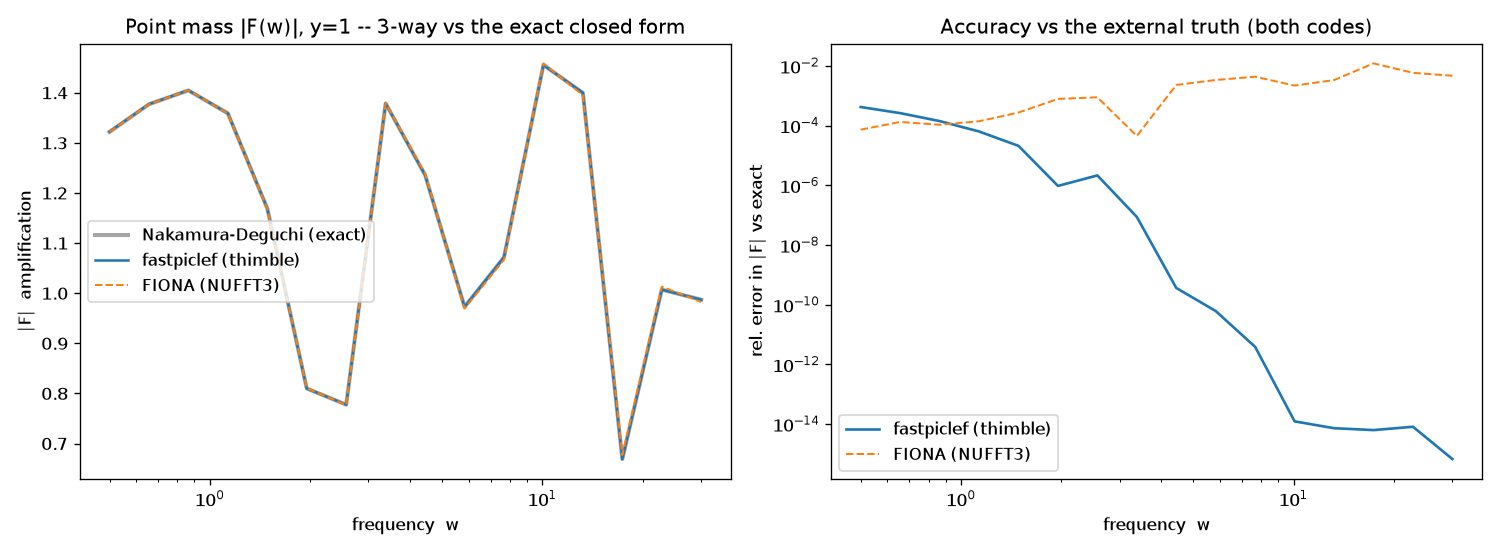
\includegraphics[width=0.98\textwidth]{freq.png}
\caption{Isolated point mass: the amplification $|F(\omega)|$ for $y=1$
(left: all codes agree at the resolution of the eye) and the relative error
against the exact Nakamura--Deguchi closed form (right).  The exact RC path
is flat at $10^{-15}$; the polar path degrades gracefully at high $\omega$
(its 1D parametrisation), and FIONA sits at $10^{-4}$--$10^{-2}$.
Figure generated by the comparison harness
(\texttt{notebooks/comparison.ipynb}; data \texttt{freq\_times.csv}).}
\label{fig:freq}
\end{figure}

\begin{figure}[t]
\centering
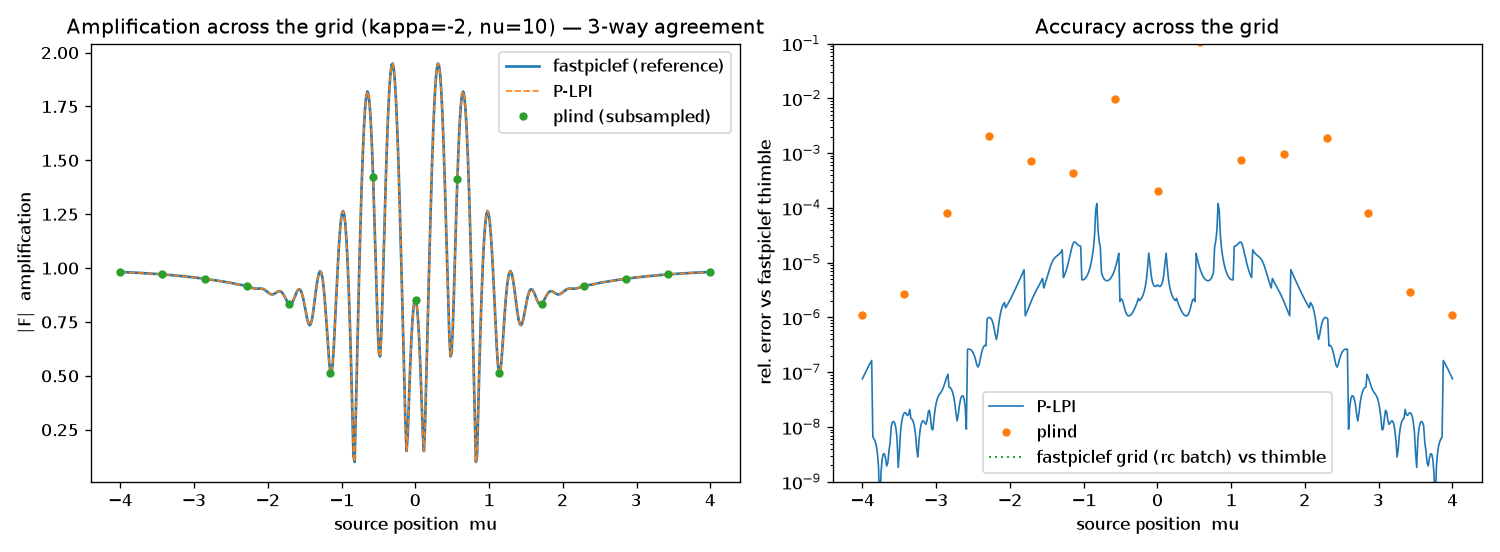
\includegraphics[width=0.98\textwidth]{grid.png}
\caption{Source sweep for a rational lens ($\kappa=-2$, $\omega=10$),
including caustic crossings: left, the amplification computed by the local
solver (reference), \texttt{P-LPI} and \texttt{plind} (subsampled); right,
each code's relative error against the reference.  The dotted line is the
local batched-grid path against the 1D thimble on the same points
($\sim10^{-9}$ agreement at the time of the run; the scalar paths agree at
$10^{-15}$-class and the batching path's floor is re-checked in the
nightly tests).}
\label{fig:grid}
\end{figure}

\subsection{Fast paths}
For the isolated lens the practical guidance is a two-line route: ND
closed form ($\sim$10\,$\mu$s) wherever $|z| = \omega y^2/2 \lesssim 10$;
the polar path above ($\sim$30\,ms at $\omega=10$, $\sim$300\,ms at
$\omega=100$); the exact 2D RC at low $\omega$ where it is exact and cheap
($\sim$0.1--0.4\,s at $\omega \le 3$).  For fields of many masses the exact
engine plus batched maps remains the production route for the science
regimes of Sec.~\ref{sec:outlook}.

% ============================================================================
\section{The time-domain view}
\label{sec:timedomain}

Frequency-domain amplifications $F(\omega)$ are one face of the physics; detectors record
arrival times.  The bridge is the impulse response,
\begin{equation}
  I(\tau) \;=\; \frac{1}{2\pi}\int \Fresnel(\omega)\,e^{-\ii\omega\tau}\,\dd\omega ,
  \label{eq:impulse}
\end{equation}
whose geometric limit is a train of pulses at the Fermat delays $\varphi_j$,
$I(\tau)\to\sum_j |\mu_j|^{1/2}e^{-\ii\pi n_j}\delta(\tau-\varphi_j)$: the images' arrival
times, their magnifications as heights, and the Morse phases as complex phases.  Because the
solver returns the exact $F(\omega)$ on any band (and the batched paths make wide sweeps
cheap), $I(\tau)$ is a two-line computation on top of the engines.  The companion notebook
\code{notebooks/time_domain.ipynb} demonstrates, for the point mass:
(i) the interference fringes of $|F(\omega)|$ with period $2\pi/\Delta\tau$ (measured $5.156$
against $5.160$ predicted at $y=0.6$, dataset: notebook outputs);
(ii) pulses at the Fermat delays with amplitudes $|\mu_j|^{1/2}$ (measured 1.199 vs 1.201 and
0.662 vs 0.665) and phases $0$ and $-\pi/2$ (the minimum and saddle Morse phases, measured
$0.008$ and $-1.587$ rad) --- the saddle image's quarter-period phase shift, rarely seen
directly;
(iii) through the caustic at $y\to0$ the two pulses merge and interfere, the merged peak
exceeding either component (5.05 versus amplitudes 3.24 and 3.08 at $y=0.05$) --- the regime
where the geometric $\delta$-comb is invalid.

Dividing by $\ii\omega$ before the transform cancels the explicit $\omega$ of
Eq.~\eqref{eq:fresnel} and yields the \emph{equal-time-delay density} of the lens plane,
\begin{equation}
  \rho(\tau) \;=\; \int \dd^2x\,\delta\bigl(\varphi(x)-\tau\bigr)
  \;=\; \oint_{\varphi=\tau}\frac{\dd\ell}{|\nabla\varphi|},
  \label{eq:delaydensity}
\end{equation}
the object the time-domain contour methods work with \cite{Ephremidze2026}: it is computable
directly in \emph{real space} (a grid histogram of the Fermat potential) and shows a step at
the minimum image's delay of height $2\pi|\mu_{\min}|^{1/2}$ (measured $7.88$ against $7.55$),
a logarithmic cusp at the saddle's delay, and the smooth quadratic-far-field background.  Both
views therefore trade the same information --- exact evaluation of $F(\omega)$ is exact
evaluation of the arrival-time structure.  The contour picture behind the density is the
pinching of the equal-delay contours at the images: the loop around the minimum shrinks to a
point (the step), the contour pinches through the saddle (the log cusp, slope
$-2\sqrt{|\mu_s|}$, measured $-1.14$ against $-1.33$), and the largest contour wraps the
mass's log branch point --- the same point where the RC construction anchors its panels.  In
the complexified problem the connection to the thimble is exact: for a holomorphic phase
$\Phi$, a thimble is a level curve of $\mathrm{Re}\,\Phi$ (the constant-phase condition),
i.e.\ the same family whose real-plane members are the delay contours, and the
$\mathrm{Im}\,\Phi$ net is its orthogonal Cauchy--Riemann partner; the notebook draws both on
the 1D Airy problem together with the solver's own traced thimbles, and checks the 1D fold
coefficient $1/\sqrt{2\varphi''}$ (measured $0.497$ against $0.500$).

\section{Limitations and outlook}
\label{sec:outlook}

\subsection{Accuracy limits}
\begin{itemize}
\item Image completeness is certified only for point-mass-only fields
  (polynomial-complete finder); the general-field finder is dense and
  residual-verified but not certified (Sec.~\ref{sec:engines}).
\item The high-$\omega$ budget covers the asymptotic error at found images,
  not missing images (same caveat).
\item The low-$\omega$ free-space subtraction currently lives in the Python
  comparison layer; the Rust path is validated to $\sim10^{-12}$ at
  $\omega = 10^{-4}$ but the subtraction polish is pending.
\item The model class boundary is exact: beyond the slit-plane analytic
  profiles (SIE, EPL, elliptical NFW, or an arbitrary potential $\psi$), the
  solver makes no claim.
\end{itemize}

\subsection{Cost limits and the many-mass no-go}
The exact engine's $\mathcal O(N^2)$ node-slot scaling was attacked during
this project with a gated research prototype of ``far-field folding''
(fold distant masses into a source shift $+$ shear $+$ global phase and
restore their micro-images by corrected stationary phase; plan:
\texttt{p42-far-field-folding.md}).  The prototype validated its full
pipeline (fold algebra exact to $2\times10^{-14}$ against the $\kappa$-free
control; micro-image finder matching the closed form to
$2.2\times10^{-14}$) but \emph{failed its accuracy gate}: diluted $N=30$
fields reached only $9\times10^{-3}$--$1.3\times10^{-2}$ at
$\omega = 1$--$3$ ($N=100$ in the science geometry: $2.4\times10^{-2}$ at
$\omega = 3$), dense fields $0.16$--$0.64$, with the failure mechanisms
identified (the micro stationary phase requires $|C|/\omega \ll 1$, false in
the science regime, and exact treatment of transition stars needs a
Taylor gap that Poisson star fields do not have).  The budget correctly
flagged the mode as invalid wherever it was inaccurate.  Two dense draws
could not even be scored: their exact-RC references failed to converge
after $6.6$\,h (error estimate $7.4$) and $75$\,min ($3.4$), so they are
excluded from the quoted ranges; those corners are provably untestable
rather than merely untested.  The exact engine,
batched maps and the high-$\omega$ hybrid therefore remain the production
route, and scalable many-mass work needs either an FMM-with-winding
(research) or explicitly approximate modes accepted by the science.

\subsection{The heuristic shortcut, measured}
\label{sec:logistic}
A cheap alternative to evaluating \eqref{eq:fresnel} is to \emph{bridge}
the two known regimes by hand: blend the geometric stationary-phase sum
$\sum_j|\mu_j|^{1/2}e^{\ii(\omega\varphi_j-\pi n_j/2)}$ (exact as
$\omega\to\infty$) with the no-lensing limit $F\to1$ through a
logistic-like window in $\log\omega$.  We implemented that competitor
(complex- and amplitude-blending variants; window
$s=1/(1+(\omega_c/\omega)^p)$) and gave it its best possible shot:
per-case fitting of $(\omega_c,p)$ against the exact solver, a single
fixed pair for the three primary cases, and a calibration-free pair.
Over $\omega\in[0.3,30]$ the best-tuned bridge bottoms out at $2.4\%$
(point mass, $y=1$), $22\%$ (macro $+$ point mass, the substructure
configuration), and $14$--$86\%$ across a caustic-approach family
($y=0.02$--$0.2$); one fixed pair costs $18$--$41\%$ and a
calibration-free $(1,2)$ window $22$--$46\%$ --- against the exact
solver's $10^{-13}$.  The failures are structural, not tuning: at the
caustic ($y=0$) the image finder returns no images at all
($F_{\mathrm{geo}}=0$) while the exact $|F|$ grows like $\sqrt{\omega}$
(the Einstein-ring stationary manifold), and wherever two images nearly
cancel the bridge inherits the spurious geometric null.  Logistic
bridging cannot stand in for the RC engine at anything like this
precision over the wave transition band; the dataset is
\texttt{comparison/results/logistic\_bridge.\{csv,md,png\}}.

\subsection{Deferred and planned}
\begin{itemize}
\item Elliptical profiles (SIE/EPL) via complex-affine quadratic forms: a
  separate branch-structure study.
\item The end-stage comparison against a heuristic logistic-bridging
  implementation of the wave/geometric transition (the project's original
  plan lists this explicitly last).
\item Notebooks demonstrating the high-$\omega$ hybrid and the ND fast path
  are pending.
\end{itemize}

% ============================================================================
\appendix

\section{Conventions}
\label{app:conv}
Throughout, lengths are in units of the reference Einstein radius and
$\omega$ is the dimensionless frequency of Eq.~\eqref{eq:omega}.  The
amplification is normalised to free space: $\Fresnel \to 1$ as $\psi \to
0$, and $|\Fresnel|^2$ is the flux ratio.  The Nakamura--Deguchi closed
form as implemented \code{(src/nd.rs)} is
\begin{equation}
  \Fresnel(\omega,y) = e^{\pi\omega/4}\,
  e^{\ii\frac{\omega}{2}\left(\ln\frac{\omega}{2}-2\phi_m\right)}\,
  \Gamma\!\left(1-\tfrac{\ii\omega}{2}\right)\,
  {}_1F_1\!\left(\tfrac{\ii\omega}{2},1;\tfrac{\ii\omega y^2}{2}\right),
\end{equation}
with $x_m = \tfrac12(y+\sqrt{y^2+4})$, $\phi_m =
\tfrac12(x_m-y)^2 - \ln x_m$, in the Takahashi--Nakamura convention.  The
code's own solvers return the un-offset normalisation of
Eq.~\eqref{eq:fresnel}; the two agree in modulus, and the complex-convention
relation ($\omega I/2\pi\ii = \Fresnel e^{\ii\omega\phi_m}$) is pinned in the
tests (\code{tests/point_mass.rs}).

\section{Dataset and code map}
\label{app:map}
\begin{center}
\small
\setlength{\tabcolsep}{4pt}
\begin{tabular}{@{}>{\raggedright\arraybackslash}p{5.4cm}>{\raggedright\arraybackslash}p{9.6cm}@{}}
\toprule
claim & dataset / artefact\\
\midrule
reference-level accuracy ($10^{-15}$-class) &
  \code{comparison/results/wolensing_compare.csv}, \code{tests/}\\
cost vs $\omega$, threading, ND comparison &
  \code{comparison/results/high_omega.csv}\\
many-mass cost, batching factor &
  \code{comparison/results/many_masses.csv}\\
head-to-head (\texttt{plind}, \texttt{P-LPI}, FIONA) &
  \code{comparison/results/summary.csv}, \texttt{grid\_times.csv},
  \texttt{freq\_times.csv}, \texttt{fiona\_grid.csv}\\
profile validation vs FIONA &
  \code{comparison/results/profiles_fiona.csv}\\
hybrid budget coverage &
  \code{comparison/results/hybrid_check.csv}\\
convergence orders, difficult cases &
  \texttt{comparison/results/convergence\_p3.\{csv,png\}},
  \texttt{difficult\_cases.\{csv,md\}}\\
many-mass folding (negative result) &
  \texttt{comparison/results/many\_masses\_fold.\{csv,md\}}\\
logistic-bridging shortcut (negative result) &
  \texttt{comparison/results/logistic\_bridge.\{csv,md,png\}}\\
all error budgets, term by term & \code{docs/error_budget.md}\\
\bottomrule
\end{tabular}
\end{center}

\section{Reproducing}
\label{app:repro}
The repository's CI script (\code{scripts/ci.sh}) builds the Rust core
with the full release test suite ($123$ tests across $15$ binaries), rebuilds
the Python bindings with \texttt{maturin}, and runs the Python wrapper
tests ($22$ tests) plus the examples build.  The comparison harness and the
reference codes live in dedicated \texttt{pixi} environments; each
comparison figure names its generating script in
\code{comparison/results/}.  The executed notebooks
(\code{notebooks/getting\_started.ipynb}, \code{notebooks/comparison.ipynb},
\code{notebooks/method.ipynb}, \code{notebooks/time\_domain.ipynb})
demonstrate the API end to end --- including the fast paths of
Sec.~\ref{sec:engines}, the self-contained visualisation of the contour
construction, the head-to-head of Sec.~\ref{sec:head2head}, and the
time-domain view of Sec.~\ref{sec:timedomain} --- with embedded outputs and
figures.  The development journal
(\texttt{Journal.typ}) records the chronological evidence trail, including
the negative results, with dataset names at every step.

\begin{thebibliography}{9}
\bibitem{DeguchiWatson1986} S.~Deguchi and W.~D. Watson,
  ``Diffraction in gravitational lensing for compact sources,''
  Astrophys.\ J.\ \textbf{307} (1986) 30.
\bibitem{Nakamura1998} T.~T. Nakamura,
  ``Gravitational lensing of gravitational waves from inspiraling
  binaries by a point mass lens,'' Phys.\ Rev.\ Lett.\ \textbf{80} (1998)
  1138.
\bibitem{TakahashiNakamura2003} R.~Takahashi and T.~T. Nakamura,
  ``Wave effects in the gravitational lensing of gravitational waves from
  chirping sources,'' Astrophys.\ J.\ \textbf{595} (2003) 1039
  [arXiv:astro-ph/0305055].
\bibitem{Feldbrugge2019} J.~Feldbrugge, U.-L. Pen and N.~Turok,
  ``Oscillatory path integrals for radio astronomy,''
  arXiv:1909.04632.
\bibitem{Jow2021} D.~L. Jow, F.~X. Lin, E.~Tyhurst and U.-L. Pen,
  ``Imaginary images and Stokes phenomena in the weak plasma lensing of
  coherent sources,'' Mon.\ Not.\ Roy.\ Astron.\ Soc.\ (2021)
  [arXiv:2103.08687].
\bibitem{Shi2024} X.~Shi,
  ``Acquiring the Lefschetz thimbles: efficient evaluation of the
  diffraction integral for lensing in wave optics,''
  arXiv:2409.12991.
\bibitem{Ephremidze2026} N.~Ephremidze, M.~Kamionkowski and C.~Dvorkin,
  ``Fast Fourier transform evaluation of the Fresnel integral for
  gravitational-wave lensing,'' arXiv:2603.12333.
\end{thebibliography}

\end{document}
